\documentclass[9pt,letter]{article}
\usepackage{lmodern}
\usepackage{amssymb,amsmath}
\usepackage{ifxetex,ifluatex}
\usepackage{fixltx2e} % provides \textsubscript
\ifnum 0\ifxetex 1\fi\ifluatex 1\fi=0 % if pdftex
  \usepackage[T1]{fontenc}
  \usepackage[utf8]{inputenc}
\else % if luatex or xelatex
  \ifxetex
    \usepackage{mathspec}
  \else
    \usepackage{fontspec}
  \fi
  \defaultfontfeatures{Ligatures=TeX,Scale=MatchLowercase}
\fi
% use upquote if available, for straight quotes in verbatim environments
\IfFileExists{upquote.sty}{\usepackage{upquote}}{}
% use microtype if available
\IfFileExists{microtype.sty}{%
\usepackage{microtype}
\UseMicrotypeSet[protrusion]{basicmath} % disable protrusion for tt fonts
}{}
\usepackage[margin=.75in]{geometry}
\usepackage{hyperref}
\hypersetup{unicode=true,
            pdftitle={A3\_tests},
            pdfauthor={Azoacha Forcheh, 20558994},
            pdfborder={0 0 0},
            breaklinks=true}
\urlstyle{same}  % don't use monospace font for urls
\usepackage{color}
\usepackage{fancyvrb}
\newcommand{\VerbBar}{|}
\newcommand{\VERB}{\Verb[commandchars=\\\{\}]}
\DefineVerbatimEnvironment{Highlighting}{Verbatim}{commandchars=\\\{\}}
% Add ',fontsize=\small' for more characters per line
\usepackage{framed}
\definecolor{shadecolor}{RGB}{248,248,248}
\newenvironment{Shaded}{\begin{snugshade}}{\end{snugshade}}
\newcommand{\KeywordTok}[1]{\textcolor[rgb]{0.13,0.29,0.53}{\textbf{#1}}}
\newcommand{\DataTypeTok}[1]{\textcolor[rgb]{0.13,0.29,0.53}{#1}}
\newcommand{\DecValTok}[1]{\textcolor[rgb]{0.00,0.00,0.81}{#1}}
\newcommand{\BaseNTok}[1]{\textcolor[rgb]{0.00,0.00,0.81}{#1}}
\newcommand{\FloatTok}[1]{\textcolor[rgb]{0.00,0.00,0.81}{#1}}
\newcommand{\ConstantTok}[1]{\textcolor[rgb]{0.00,0.00,0.00}{#1}}
\newcommand{\CharTok}[1]{\textcolor[rgb]{0.31,0.60,0.02}{#1}}
\newcommand{\SpecialCharTok}[1]{\textcolor[rgb]{0.00,0.00,0.00}{#1}}
\newcommand{\StringTok}[1]{\textcolor[rgb]{0.31,0.60,0.02}{#1}}
\newcommand{\VerbatimStringTok}[1]{\textcolor[rgb]{0.31,0.60,0.02}{#1}}
\newcommand{\SpecialStringTok}[1]{\textcolor[rgb]{0.31,0.60,0.02}{#1}}
\newcommand{\ImportTok}[1]{#1}
\newcommand{\CommentTok}[1]{\textcolor[rgb]{0.56,0.35,0.01}{\textit{#1}}}
\newcommand{\DocumentationTok}[1]{\textcolor[rgb]{0.56,0.35,0.01}{\textbf{\textit{#1}}}}
\newcommand{\AnnotationTok}[1]{\textcolor[rgb]{0.56,0.35,0.01}{\textbf{\textit{#1}}}}
\newcommand{\CommentVarTok}[1]{\textcolor[rgb]{0.56,0.35,0.01}{\textbf{\textit{#1}}}}
\newcommand{\OtherTok}[1]{\textcolor[rgb]{0.56,0.35,0.01}{#1}}
\newcommand{\FunctionTok}[1]{\textcolor[rgb]{0.00,0.00,0.00}{#1}}
\newcommand{\VariableTok}[1]{\textcolor[rgb]{0.00,0.00,0.00}{#1}}
\newcommand{\ControlFlowTok}[1]{\textcolor[rgb]{0.13,0.29,0.53}{\textbf{#1}}}
\newcommand{\OperatorTok}[1]{\textcolor[rgb]{0.81,0.36,0.00}{\textbf{#1}}}
\newcommand{\BuiltInTok}[1]{#1}
\newcommand{\ExtensionTok}[1]{#1}
\newcommand{\PreprocessorTok}[1]{\textcolor[rgb]{0.56,0.35,0.01}{\textit{#1}}}
\newcommand{\AttributeTok}[1]{\textcolor[rgb]{0.77,0.63,0.00}{#1}}
\newcommand{\RegionMarkerTok}[1]{#1}
\newcommand{\InformationTok}[1]{\textcolor[rgb]{0.56,0.35,0.01}{\textbf{\textit{#1}}}}
\newcommand{\WarningTok}[1]{\textcolor[rgb]{0.56,0.35,0.01}{\textbf{\textit{#1}}}}
\newcommand{\AlertTok}[1]{\textcolor[rgb]{0.94,0.16,0.16}{#1}}
\newcommand{\ErrorTok}[1]{\textcolor[rgb]{0.64,0.00,0.00}{\textbf{#1}}}
\newcommand{\NormalTok}[1]{#1}
\usepackage{graphicx,grffile}
\makeatletter
\def\maxwidth{\ifdim\Gin@nat@width>\linewidth\linewidth\else\Gin@nat@width\fi}
\def\maxheight{\ifdim\Gin@nat@height>\textheight\textheight\else\Gin@nat@height\fi}
\makeatother
% Scale images if necessary, so that they will not overflow the page
% margins by default, and it is still possible to overwrite the defaults
% using explicit options in \includegraphics[width, height, ...]{}
\setkeys{Gin}{width=\maxwidth,height=\maxheight,keepaspectratio}
\IfFileExists{parskip.sty}{%
\usepackage{parskip}
}{% else
\setlength{\parindent}{0pt}
\setlength{\parskip}{6pt plus 2pt minus 1pt}
}
\setlength{\emergencystretch}{3em}  % prevent overfull lines
\providecommand{\tightlist}{%
  \setlength{\itemsep}{0pt}\setlength{\parskip}{0pt}}
\setcounter{secnumdepth}{0}
% Redefines (sub)paragraphs to behave more like sections
\ifx\paragraph\undefined\else
\let\oldparagraph\paragraph
\renewcommand{\paragraph}[1]{\oldparagraph{#1}\mbox{}}
\fi
\ifx\subparagraph\undefined\else
\let\oldsubparagraph\subparagraph
\renewcommand{\subparagraph}[1]{\oldsubparagraph{#1}\mbox{}}
\fi

%%% Use protect on footnotes to avoid problems with footnotes in titles
\let\rmarkdownfootnote\footnote%
\def\footnote{\protect\rmarkdownfootnote}

%%% Change title format to be more compact
\usepackage{titling}

% Create subtitle command for use in maketitle
\newcommand{\subtitle}[1]{
  \posttitle{
    \begin{center}\large#1\end{center}
    }
}

\setlength{\droptitle}{-2em}
  \title{A3\_tests}
  \pretitle{\vspace{\droptitle}\centering\huge}
  \posttitle{\par}
  \author{Azoacha Forcheh, 20558994}
  \preauthor{\centering\large\emph}
  \postauthor{\par}
  \date{}
  \predate{}\postdate{}

\usepackage{graphicx}
\usepackage{color}
\usepackage{enumitem}
\newcommand{\benum}{\begin{enumerate}}
\newcommand{\eenum}{\end{enumerate}}
\newcommand{\bitem}{\begin{itemize}}
\newcommand{\eitem}{\end{itemize}}

\begin{document}
\maketitle

\benum
\item Have a look at the video \url{https://youtu.be/HEheh1BH34Q} which
compares the sizes of various astronomical bodies. The video tries to
give some sense of the comparative size of these bodies.

In the \texttt{R} code folder there is a file called \texttt{stars.R}
that contains measurements of the radius in kilometres of several
astronomical bodies in our solar system (in a vector called
\texttt{solarSystemRadii}) and of the radius of many stars as measured
in numbers of solar radii (in a vector called \texttt{starRadii}). Load
this file into \texttt{R} (use \texttt{source("directory/stars.R")} with
the \texttt{directory} changed to wherever you put the file
\texttt{stars.R}). For example:

\begin{Shaded}
\begin{Highlighting}[]
\KeywordTok{source}\NormalTok{(}\StringTok{"./stars.R"}\NormalTok{)}
\CommentTok{# Have a look at the contents of each}
\KeywordTok{head}\NormalTok{(solarSystemRadii)}
\end{Highlighting}
\end{Shaded}

\begin{verbatim}
##         radius
## Sun     696000
## Jupiter  69911
## Saturn   58232
## Uranus   25362
## Neptune  24622
## Earth     6371
\end{verbatim}

\begin{Shaded}
\begin{Highlighting}[]
\KeywordTok{head}\NormalTok{(starRadii)}
\end{Highlighting}
\end{Shaded}

\begin{verbatim}
##                    radius
## binarystarvvcephei   1900
## v354cephei           1520
## mucephei             1420
## kycygni              1420
## v509cassiopeiae       900
## v838monocerotis      1570
\end{verbatim}

\benum
\item In the video, the relative size of the planets is encoded in at
least three ways.

\benum
\item \textbf{(3 marks)} Name them.

Volume, position along a common scale, length

\item 

\textbf{(3 marks)} According to Stevens's law, which encoding is most
reliably encoded? Which least? (Justify your answers by appeal to this
law.)

According to Steven's law, length is most reliable encoding as it
creates the smallest bias when encoding the relative size of the
planets, which is due to its higher empirically observed range of values
\(0.9 \le \beta \le 1.1\), making \(p(x) \approx cx\). The least
reliable encoding is volume, which has the largest bias of the 3 when
encoding the relative size of the planets, due to its lower empirically
observed range of values \(0.5 \le \beta \le 0.8\).

\item 

\textbf{(1 marks)} How might position along a common scale have been
used instead? As the bodies being considered were all spheres, the
position along a common scale could have been used to display and
compare the radii (a measurement of length) of the bodies instead of the
volumes, which is only dependent on the radii and is a less accurate
encoding according to Steven's law.

\eenum

\item 

For the \texttt{solarSystemRadii} data:

Here you are going to draw the various astronomical bodies in our solar
system in much the same way as they appear in that video. You will be
making use of the \texttt{grid} package (as seen in previous
assignments).

You will need to recall a few things about \texttt{grid}. As before, you
will just be drawing circles to represent the various bodies so the
function \texttt{gridcircle(..)} will be used. Remember that (so far
anyway) that you are always drawing within a {[}0,1{]} rectangle do that
everything you draw will need to be translated to this range
(e.g.~dividing all radii by the maximum diameter will allow all circles
will fit within the unit square when centred at (0.5, 0.5).

You will also need a palette of colours, one for each body. How to
construct a palette of was described during an earlier lecture on
numbers and made available on the course web page.

The code below should give you some idea of what is possible. (See
help(\ldots{}) on any function to explore more parameter choices.)

\begin{Shaded}
\begin{Highlighting}[]
\KeywordTok{library}\NormalTok{(grid)}
\KeywordTok{library}\NormalTok{(colorspace)}
\NormalTok{cols <-}\StringTok{ }\KeywordTok{rainbow_hcl}\NormalTok{(}\DataTypeTok{n=}\DecValTok{5}\NormalTok{, }\DataTypeTok{c=}\DecValTok{100}\NormalTok{)  }\CommentTok{# 5 different colours having chroma = 100}

\KeywordTok{grid.newpage}\NormalTok{()}
\ControlFlowTok{for}\NormalTok{ (i }\ControlFlowTok{in} \DecValTok{1}\OperatorTok{:}\DecValTok{5}\NormalTok{) \{}
  \KeywordTok{grid.circle}\NormalTok{(}\DataTypeTok{x=}\FloatTok{0.5}\NormalTok{,}
              \DataTypeTok{y=}\FloatTok{0.5}\NormalTok{,}
              \DataTypeTok{r =}\NormalTok{ (}\DecValTok{6}\OperatorTok{-}\NormalTok{i)}\OperatorTok{/}\DecValTok{10}\NormalTok{,}
              \DataTypeTok{gp=}\KeywordTok{gpar}\NormalTok{(}\DataTypeTok{fill=}\KeywordTok{adjustcolor}\NormalTok{(cols[i], }\DataTypeTok{alpha.f =} \FloatTok{0.5}\NormalTok{))}
\NormalTok{  )}
\NormalTok{\}}
\CommentTok{# Now add a label and an arrow}
\NormalTok{xcentre <-}\StringTok{ }\FloatTok{0.5}
\NormalTok{ycentre <-}\StringTok{ }\FloatTok{0.5}
\NormalTok{degrees <-}\StringTok{ }\DecValTok{45}
\NormalTok{radians <-}\StringTok{ }\NormalTok{pi }\OperatorTok{*}\StringTok{ }\NormalTok{degrees }\OperatorTok{/}\StringTok{ }\DecValTok{180}
\NormalTok{arrowLength <-}\StringTok{ }\FloatTok{0.5} 
\NormalTok{xarrowFrom <-}\StringTok{ }\NormalTok{xcentre }\OperatorTok{+}\StringTok{ }\NormalTok{arrowLength }\OperatorTok{*}\StringTok{ }\KeywordTok{cos}\NormalTok{(radians)}
\NormalTok{yarrowFrom <-}\StringTok{ }\NormalTok{ycentre }\OperatorTok{+}\StringTok{ }\NormalTok{arrowLength }\OperatorTok{*}\StringTok{ }\KeywordTok{sin}\NormalTok{(radians)}
\NormalTok{xarrowTo <-}\StringTok{ }\NormalTok{xcentre }
\NormalTok{yarrowTo <-}\StringTok{ }\NormalTok{ycentre}
\CommentTok{# draw arrow}
\KeywordTok{grid.lines}\NormalTok{(}\DataTypeTok{x=}\KeywordTok{c}\NormalTok{(xarrowFrom, xarrowTo), }\DataTypeTok{y=}\KeywordTok{c}\NormalTok{(yarrowFrom, yarrowTo), }
           \DataTypeTok{arrow=}\KeywordTok{arrow}\NormalTok{(),}
           \DataTypeTok{gp =} \KeywordTok{gpar}\NormalTok{(}\DataTypeTok{col=}\StringTok{"black"}\NormalTok{, }\DataTypeTok{lwd=}\DecValTok{1}\NormalTok{, }\DataTypeTok{lty =} \DecValTok{1}\NormalTok{))}

\NormalTok{delta <-}\StringTok{ }\FloatTok{0.01}
\NormalTok{xText <-}\StringTok{ }\NormalTok{xarrowFrom }\OperatorTok{+}\StringTok{ }\NormalTok{delta }\OperatorTok{*}\StringTok{ }\KeywordTok{cos}\NormalTok{(radians)}
\NormalTok{yText <-}\StringTok{ }\NormalTok{yarrowFrom }\OperatorTok{+}\StringTok{ }\NormalTok{delta }\OperatorTok{*}\StringTok{ }\KeywordTok{sin}\NormalTok{(radians)}
\KeywordTok{grid.text}\NormalTok{(}\StringTok{"Centre"}\NormalTok{, }\DataTypeTok{x=}\NormalTok{ xText, }\DataTypeTok{y=}\NormalTok{ yText,}
          \DataTypeTok{just=}\StringTok{"left"}\NormalTok{, }\DataTypeTok{rot =}\NormalTok{ degrees,}
          \DataTypeTok{gp =} \KeywordTok{gpar}\NormalTok{(}\DataTypeTok{col=}\StringTok{"black"}\NormalTok{))}
\end{Highlighting}
\end{Shaded}

\begin{center}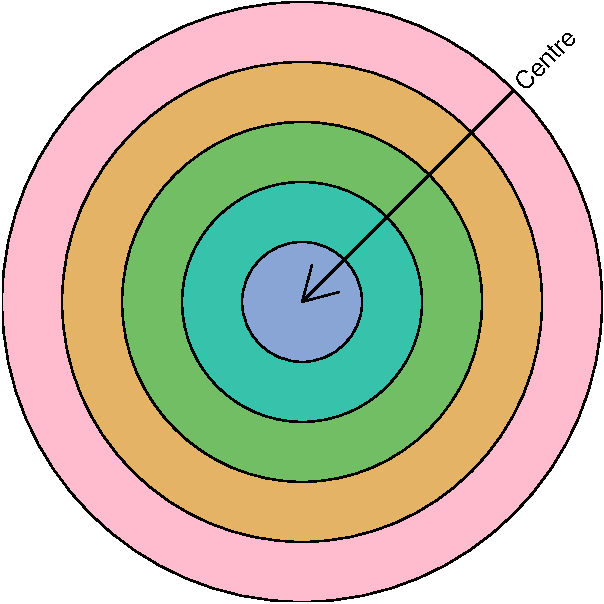
\includegraphics{a3_tests_files/figure-latex/unnamed-chunk-2-1} \end{center}

These functions (and the \texttt{grid} package) are to be used to
address the following questions.

\benum
\item \textbf{(5 marks)} Represent each body by a circle whose radius is
proportional to the radius in kilometres of that body (use the radius of
the sun as the maximum possible radius in the display).

Align the circles so that they are all centred on (0.5, 0.5). Label each
of the three largest bodies (excluding the sun) on the plot. Show your
code and the picture produced.

\textbf{IMPORTANT:} you need to maintain an aspect ratio of 1 so begin
your \texttt{r} code chunks in \texttt{Rmarkdown} with something like
\texttt{\{r,\ fig.align="center",\ fig.width=4,\ fig.height=4\}}

\begin{Shaded}
\begin{Highlighting}[]
\KeywordTok{library}\NormalTok{(grid)}
\KeywordTok{library}\NormalTok{(colorspace)}

\NormalTok{xcentre =}\StringTok{ }\FloatTok{0.5}
\NormalTok{ycentre =}\StringTok{ }\FloatTok{0.5}
\NormalTok{cols =}\StringTok{ }\KeywordTok{rainbow_hcl}\NormalTok{(}\DecValTok{6}\NormalTok{, }\DataTypeTok{c =} \DecValTok{100}\NormalTok{)}
\NormalTok{n =}\StringTok{ }\KeywordTok{dim}\NormalTok{(solarSystemRadii)[}\DecValTok{1}\NormalTok{]}
\NormalTok{max_diam =}\StringTok{ }\NormalTok{solarSystemRadii[}\StringTok{'Sun'}\NormalTok{,]}
  
\KeywordTok{grid.newpage}\NormalTok{()}
\ControlFlowTok{for}\NormalTok{ (i }\ControlFlowTok{in} \DecValTok{1}\OperatorTok{:}\NormalTok{n) \{}
  \KeywordTok{grid.circle}\NormalTok{(}\DataTypeTok{x=}\NormalTok{xcentre,}
              \DataTypeTok{y=}\NormalTok{ycentre,}
              \DataTypeTok{r =}\NormalTok{ (solarSystemRadii[i,]}\OperatorTok{/}\NormalTok{max_diam)}\OperatorTok{/}\DecValTok{2}\NormalTok{,}
              \DataTypeTok{gp=}\KeywordTok{gpar}\NormalTok{(}\DataTypeTok{fill=}\KeywordTok{adjustcolor}\NormalTok{(cols[i], }\DataTypeTok{alpha.f =} \FloatTok{0.5}\NormalTok{))}
\NormalTok{  )}
\NormalTok{\}}

\NormalTok{degs =}\StringTok{ }\KeywordTok{c}\NormalTok{(}\DecValTok{45}\NormalTok{, }\DecValTok{135}\NormalTok{, }\DecValTok{315}\NormalTok{)}
\ControlFlowTok{for}\NormalTok{ (i }\ControlFlowTok{in} \DecValTok{2}\OperatorTok{:}\DecValTok{4}\NormalTok{) \{}
\NormalTok{  degrees =}\StringTok{ }\NormalTok{degs[i}\OperatorTok{-}\DecValTok{1}\NormalTok{]}
\NormalTok{  radians =}\StringTok{ }\NormalTok{pi }\OperatorTok{*}\StringTok{ }\NormalTok{degrees }\OperatorTok{/}\StringTok{ }\DecValTok{180}
\NormalTok{  arrowLength =}\StringTok{ }\FloatTok{0.5} 
\NormalTok{  xarrowFrom =}\StringTok{ }\NormalTok{xcentre }\OperatorTok{+}\StringTok{ }\NormalTok{arrowLength }\OperatorTok{*}\StringTok{ }\KeywordTok{cos}\NormalTok{(radians)}
\NormalTok{  yarrowFrom =}\StringTok{ }\NormalTok{ycentre }\OperatorTok{+}\StringTok{ }\NormalTok{arrowLength }\OperatorTok{*}\StringTok{ }\KeywordTok{sin}\NormalTok{(radians)}
  
  \ControlFlowTok{if}\NormalTok{ (degrees }\OperatorTok{==}\StringTok{ }\DecValTok{135}\NormalTok{) \{}
\NormalTok{    xarrowTo =}\StringTok{ }\NormalTok{xcentre }\OperatorTok{-}\StringTok{ }\NormalTok{(solarSystemRadii[i,]}\OperatorTok{/}\NormalTok{max_diam)}\OperatorTok{/}\DecValTok{2}
\NormalTok{  \} }\ControlFlowTok{else}\NormalTok{ \{}
\NormalTok{    xarrowTo =}\StringTok{ }\NormalTok{xcentre }\OperatorTok{+}\StringTok{ }\NormalTok{(solarSystemRadii[i,]}\OperatorTok{/}\NormalTok{max_diam)}\OperatorTok{/}\DecValTok{2}
\NormalTok{  \}}
  
\NormalTok{  yarrowTo =}\StringTok{ }\NormalTok{ycentre}
  \CommentTok{# draw arrow}
  \KeywordTok{grid.lines}\NormalTok{(}\DataTypeTok{x=}\KeywordTok{c}\NormalTok{(xarrowFrom, xarrowTo), }\DataTypeTok{y=}\KeywordTok{c}\NormalTok{(yarrowFrom, yarrowTo), }
             \DataTypeTok{arrow=}\KeywordTok{arrow}\NormalTok{(),}
             \DataTypeTok{gp =} \KeywordTok{gpar}\NormalTok{(}\DataTypeTok{col=}\StringTok{"black"}\NormalTok{, }\DataTypeTok{lwd=}\DecValTok{1}\NormalTok{, }\DataTypeTok{lty =} \DecValTok{1}\NormalTok{))}
  
\NormalTok{  delta =}\StringTok{ }\FloatTok{0.01}
\NormalTok{  xText =}\StringTok{ }\NormalTok{xarrowFrom }\OperatorTok{+}\StringTok{ }\NormalTok{delta }\OperatorTok{*}\StringTok{ }\KeywordTok{cos}\NormalTok{(radians)}
\NormalTok{  yText =}\StringTok{ }\NormalTok{yarrowFrom }\OperatorTok{+}\StringTok{ }\NormalTok{delta }\OperatorTok{*}\StringTok{ }\KeywordTok{sin}\NormalTok{(radians)}
  
\NormalTok{  body_name =}\StringTok{ }\KeywordTok{rownames}\NormalTok{(solarSystemRadii)[i]}
  \KeywordTok{grid.text}\NormalTok{(body_name, }\DataTypeTok{x=}\NormalTok{ xText, }\DataTypeTok{y=}\NormalTok{ yText,}
            \DataTypeTok{just=}\StringTok{"left"}\NormalTok{, }\DataTypeTok{rot =}\NormalTok{ degrees,}
            \DataTypeTok{gp =} \KeywordTok{gpar}\NormalTok{(}\DataTypeTok{col=}\StringTok{"black"}\NormalTok{))}
\NormalTok{\}}
\end{Highlighting}
\end{Shaded}

\begin{center}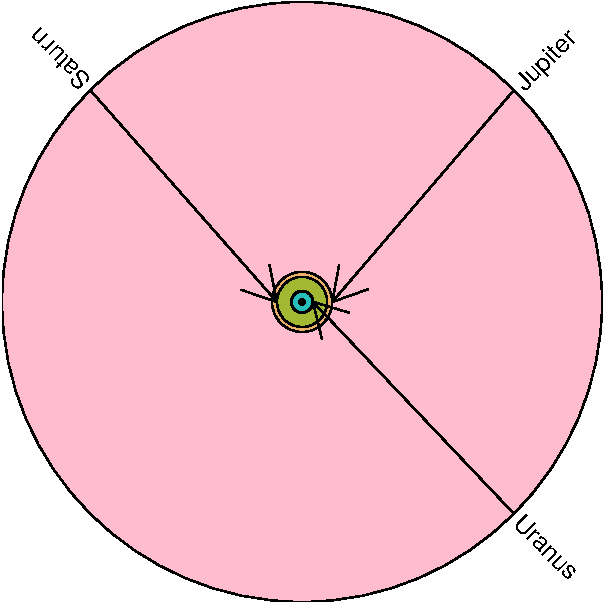
\includegraphics{a3_tests_files/figure-latex/unnamed-chunk-3-1} \end{center}

\item 

\textbf{(2 marks)} Briefly comment on how easily it is to compare the
relative sizes of Uranus to Saturn? Of Saturn to Jupiter? Of Jupiter to
the Sun? How about comparing Uranus to the Earth or the Moon?

Because the two circles representing the planets are both relatively
large and are overlaid immediately (i.e.~with no other circle between
the two) over each other, and because the colors of the circles are
diverging, it is easy to see that Uranus is much smaller than Saturn as
we can still see much of the area of the circle representing Saturn.
However, it is difficult to determine by what proportion this difference
is as we comparing the two via their areas.

For Saturn and Jupiter, it is once again easy to compare the two planets
for the exact reasons mentioned above, with it being easy to determine
that Saturn is slightly larger than Jupiter. The same applies for
comparing Jupiter to the Sun, though it is harder to make this
comparison and most of Jupiter is not visible under the overlaying
circles.

Due to the Moon and Earth being significantly smaller than the Sun, they
are very difficult to see and compare with any of the other bodies. One
can tell that the Moon and Earth are smaller than Uranus, but it is
extremely difficult to determine the ratio of difference.

\item 

\textbf{(4 marks)} According to Stevens's law, what is the range of
values we might expect for the ratio of the areas (smaller to larger) of
each of the above comparisons? How do these compare to the ratio of
actual areas?

\[
\begin{array}{rll}
\text{Uranus vs. Saturn} &:& \displaystyle [(\frac{25362^2\pi}{58232^2\pi})^{0.9}, (\frac{25362^2\pi}{58232^2\pi})^{0.6}] = [0.2239955, 0.3688299]\\
\text{Saturn vs. Jupiter} &:& \displaystyle [(\frac{58232^2\pi}{69911^2\pi})^{0.9}, (\frac{58232^2\pi}{69911^2\pi})^{0.6}] = [0.7196298, 0.8030442]\\
\text{Jupiter vs. the Sun} &:& \displaystyle [(\frac{69911^2\pi}{696000^2\pi})^{0.9}, (\frac{69911^2\pi}{696000^2\pi})^{0.6}] = [0.01597663,0.06343421]\\
\text{Earth vs. Uranus} &:& \displaystyle [(\frac{6371^2\pi}{25362^2\pi})^{0.9}, (\frac{6371^2\pi}{25362^2\pi})^{0.6}] = [0.08318469, 0.1905588]\\
\text{The Moon vs. Uranus} &:& \displaystyle [(\frac{1737.1^2\pi}{25362^2\pi})^{0.9}, (\frac{1737.1^2\pi}{25362^2\pi})^{0.6}] = [0.00796984, 0.0398994]\\
\end{array}
\]

In comparison, the actual ratios are: \[
\begin{array}{rll}
\text{Uranus vs. Saturn} &:& 0.1896896\\
\text{Saturn vs. Jupiter} &:& 0.6937969\\
\text{Jupiter vs. the Sun} &:& 0.01008957\\
\text{Earth vs. Uranus} &:& 0.004691186\\
\text{The Moon vs. Uranus} &:& 0.06310274\\
\end{array}
\]

Every one of the ratio of actual areas falls outside and to the left of
the calculated ranges for the ratios. The demonstrates the bias and
reduced accuracy of using area as a visual encoding of magnititude.

\item 

\textbf{(5 marks)} Consider now all of the bodies in the solar system
\textbf{excluding the sun}. Using the \texttt{grid} package and
\texttt{grid.circle(...)} etc. lay out all of the remaining bodies from
the smallest at the left to the largest at the right with their centres
all at \(y=0.5\) but locate them so that they do not overlap. Have the
radius of each circles be proportional to the true radius of that body.
Mark the Earth, Uranus, Saturn, Jupiter on the plot.

Show your code and your output. Some functions you might find useful are
\texttt{order(...)} to determine the order of values and possibly
\texttt{\%in\%} as in \texttt{"foo"\ \%in\%\ c("foo",\ "bar")} will
return \texttt{TRUE} if the string \texttt{"foo"} can be found in the
vector \texttt{c("foo",\ "bar")}; the latter may be helpful in deciding
whether to label or not.

\begin{Shaded}
\begin{Highlighting}[]
\NormalTok{cols =}\StringTok{ }\KeywordTok{rainbow_hcl}\NormalTok{(n}\OperatorTok{-}\DecValTok{1}\NormalTok{)}

\NormalTok{asc_order =}\StringTok{ }\KeywordTok{order}\NormalTok{(solarSystemRadii)}
\NormalTok{planets =}\StringTok{ }\NormalTok{solarSystemRadii[asc_order[}\OperatorTok{!}\StringTok{ }\NormalTok{asc_order }\OperatorTok\StringTok{ }\KeywordTok{c}\NormalTok{(}\DecValTok{1}\NormalTok{)],]}
\NormalTok{planet_names =}\StringTok{ }\KeywordTok{rownames}\NormalTok{(solarSystemRadii)[asc_order[}\OperatorTok{!}\StringTok{ }\NormalTok{asc_order }\OperatorTok\StringTok{ }\KeywordTok{c}\NormalTok{(}\DecValTok{1}\NormalTok{)]]}
\NormalTok{total_length =}\StringTok{ }\DecValTok{2}\OperatorTok{*}\KeywordTok{sum}\NormalTok{(planets)}\OperatorTok{+}\FloatTok{0.08}
\NormalTok{planetsr =}\StringTok{ }\NormalTok{planets}\OperatorTok{/}\NormalTok{total_length}

\NormalTok{xcenters =}\StringTok{ }\KeywordTok{replicate}\NormalTok{(n}\OperatorTok{-}\DecValTok{1}\NormalTok{, }\DecValTok{0}\NormalTok{)}
\ControlFlowTok{for}\NormalTok{ (i }\ControlFlowTok{in} \DecValTok{1}\OperatorTok{:}\NormalTok{(n}\OperatorTok{-}\DecValTok{1}\NormalTok{)) \{}
\NormalTok{  xcenters[i] =}\StringTok{ }\NormalTok{(}\DecValTok{2}\OperatorTok{*}\KeywordTok{sum}\NormalTok{(planetsr[}\DecValTok{1}\OperatorTok{:}\NormalTok{i}\OperatorTok{-}\DecValTok{1}\NormalTok{])) }\OperatorTok{+}\StringTok{ }\NormalTok{planetsr[i]}
\NormalTok{\}}

\KeywordTok{grid.newpage}\NormalTok{()}
\NormalTok{xcenter =}\StringTok{ }\DecValTok{0}
\NormalTok{ycenter =}\StringTok{ }\FloatTok{0.5}

\ControlFlowTok{for}\NormalTok{ (i }\ControlFlowTok{in} \DecValTok{1}\OperatorTok{:}\NormalTok{(n}\OperatorTok{-}\DecValTok{1}\NormalTok{)) \{}
  \KeywordTok{grid.circle}\NormalTok{(}\DataTypeTok{x=}\NormalTok{xcenters[i],}
              \DataTypeTok{y=}\NormalTok{ycenter,}
              \DataTypeTok{r =}\NormalTok{ planetsr[i],}
              \DataTypeTok{gp=}\KeywordTok{gpar}\NormalTok{(}\DataTypeTok{fill=}\KeywordTok{adjustcolor}\NormalTok{(cols[i], }\DataTypeTok{alpha.f =} \FloatTok{0.5}\NormalTok{)))}
  
\NormalTok{  body_name =}\StringTok{ }\NormalTok{planet_names[i]}
  \ControlFlowTok{if}\NormalTok{ (body_name }\OperatorTok\StringTok{ }\KeywordTok{c}\NormalTok{(}\StringTok{'Earth'}\NormalTok{, }\StringTok{'Uranus'}\NormalTok{, }\StringTok{'Saturn'}\NormalTok{, }\StringTok{'Jupiter'}\NormalTok{)) \{}
    \KeywordTok{grid.text}\NormalTok{(body_name, }\DataTypeTok{x=}\NormalTok{xcenters[i], }\DataTypeTok{y=}\FloatTok{0.09}\NormalTok{,}
              \DataTypeTok{just=}\StringTok{"left"}\NormalTok{,}
              \DataTypeTok{gp =} \KeywordTok{gpar}\NormalTok{(}\DataTypeTok{col=}\StringTok{"black"}\NormalTok{))}
\NormalTok{  \}}
\NormalTok{\}}
\end{Highlighting}
\end{Shaded}

\begin{center}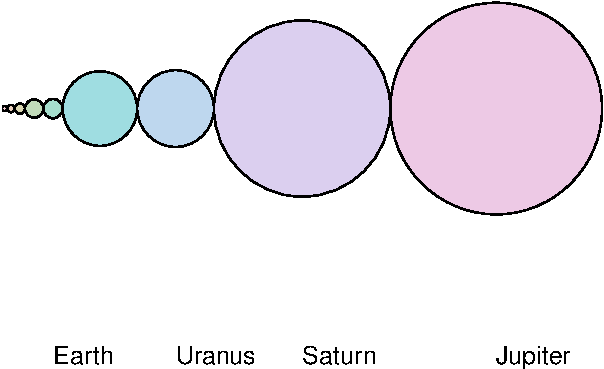
\includegraphics{a3_tests_files/figure-latex/unnamed-chunk-4-1} \end{center}

\eenum      

\item 

For the \texttt{stars} data, \benum
\item \textbf{(3 marks)} Construct a quantile plot of the radii of the
\texttt{stars}. Describe whatever patterns you see in the data.

\begin{Shaded}
\begin{Highlighting}[]
\NormalTok{n =}\StringTok{ }\KeywordTok{dim}\NormalTok{(starRadii)[}\DecValTok{1}\NormalTok{]}
\NormalTok{p =}\StringTok{ }\KeywordTok{ppoints}\NormalTok{(n)}
\KeywordTok{plot}\NormalTok{(}\DataTypeTok{x =}\NormalTok{ p, }\DataTypeTok{y=}\NormalTok{starRadii[,], }
      \DataTypeTok{type=}\StringTok{"o"}\NormalTok{, }\DataTypeTok{lwd=}\DecValTok{2}\NormalTok{, }\DataTypeTok{col=}\StringTok{"grey50"}\NormalTok{,}
      \DataTypeTok{xlab=}\StringTok{"p"}\NormalTok{, }\DataTypeTok{ylab=}\StringTok{"Radius"}\NormalTok{,}
      \DataTypeTok{main=}\StringTok{"Quantile Plot of Stars' Radii"}\NormalTok{,}
      \DataTypeTok{xlim =}\KeywordTok{c}\NormalTok{(}\DecValTok{0}\NormalTok{,}\DecValTok{1}\NormalTok{))}
\end{Highlighting}
\end{Shaded}

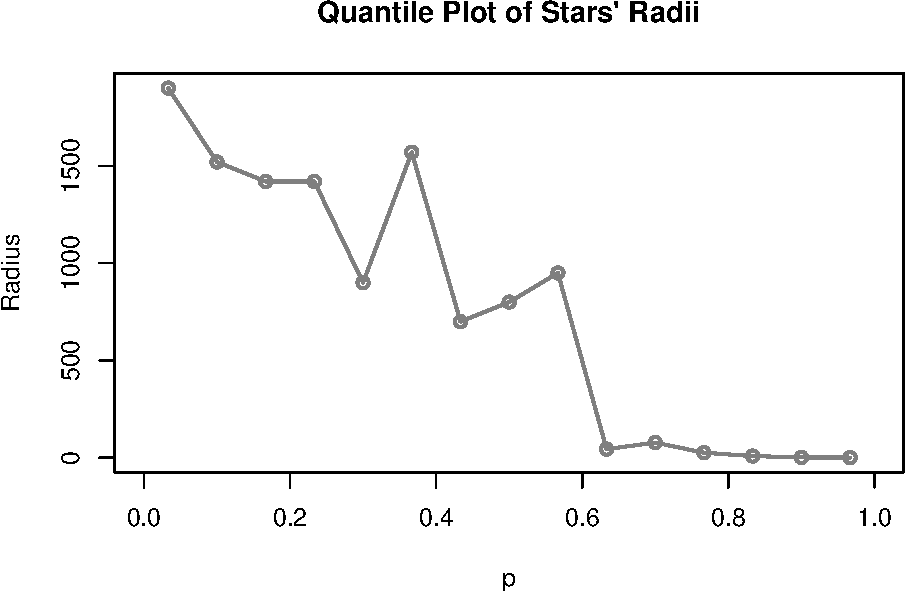
\includegraphics{a3_tests_files/figure-latex/unnamed-chunk-5-1.pdf}

\item 

\textbf{(3 marks)} Construct a quantile plot of the volume of the
\texttt{stars}. (Recall: the volume of a sphere is
\(\frac{4}{3}\pi r^3\).) Describe whatever patterns you see in the data.

\begin{Shaded}
\begin{Highlighting}[]
\NormalTok{starVolumes =}\StringTok{ }\DecValTok{4}\OperatorTok{*}\NormalTok{(starRadii[,]}\OperatorTok{^}\DecValTok{3}\NormalTok{)}\OperatorTok{/}\DecValTok{3}
\KeywordTok{plot}\NormalTok{(}\DataTypeTok{x =}\NormalTok{ p, }\DataTypeTok{y=}\NormalTok{starVolumes, }
      \DataTypeTok{type=}\StringTok{"o"}\NormalTok{, }\DataTypeTok{lwd=}\DecValTok{2}\NormalTok{, }\DataTypeTok{col=}\StringTok{"grey50"}\NormalTok{,}
      \DataTypeTok{xlab=}\StringTok{"p"}\NormalTok{, }\DataTypeTok{ylab=}\StringTok{"Volume"}\NormalTok{,}
      \DataTypeTok{main=}\StringTok{"Quantile Plot of Stars' Volumes"}\NormalTok{,}
      \DataTypeTok{xlim =}\KeywordTok{c}\NormalTok{(}\DecValTok{0}\NormalTok{,}\DecValTok{1}\NormalTok{))}
\end{Highlighting}
\end{Shaded}

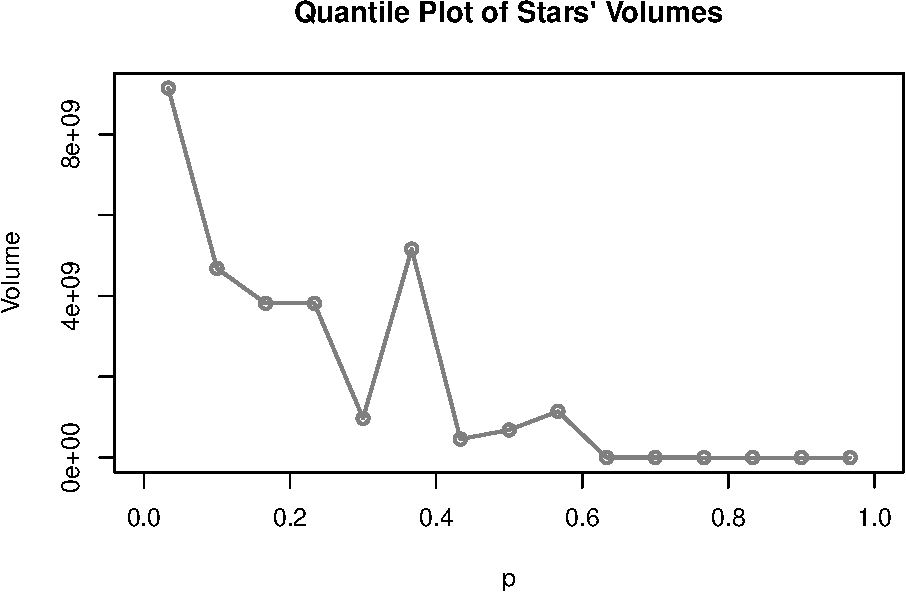
\includegraphics{a3_tests_files/figure-latex/unnamed-chunk-6-1.pdf}
\item \textbf{(2 marks)} How do these two summaries differ?

\item 

\textbf{(3 marks)} Construct a quantile plot of the base 10 logarithms
of the stellar radii. Describe whatever patterns you see in the data.

\begin{Shaded}
\begin{Highlighting}[]
\NormalTok{starLogs =}\StringTok{ }\KeywordTok{log}\NormalTok{(starRadii[,], }\DataTypeTok{base=}\DecValTok{10}\NormalTok{)}
\KeywordTok{plot}\NormalTok{(}\DataTypeTok{x =}\NormalTok{ p, }\DataTypeTok{y=}\NormalTok{starLogs, }
      \DataTypeTok{type=}\StringTok{"o"}\NormalTok{, }\DataTypeTok{lwd=}\DecValTok{2}\NormalTok{, }\DataTypeTok{col=}\StringTok{"grey50"}\NormalTok{,}
      \DataTypeTok{xlab=}\StringTok{"p"}\NormalTok{, }\DataTypeTok{ylab=}\StringTok{"Volume"}\NormalTok{,}
      \DataTypeTok{main=}\StringTok{"Quantile Plot of Stars' Base-10 Logarithms"}\NormalTok{,}
      \DataTypeTok{xlim =}\KeywordTok{c}\NormalTok{(}\DecValTok{0}\NormalTok{,}\DecValTok{1}\NormalTok{))}
\end{Highlighting}
\end{Shaded}

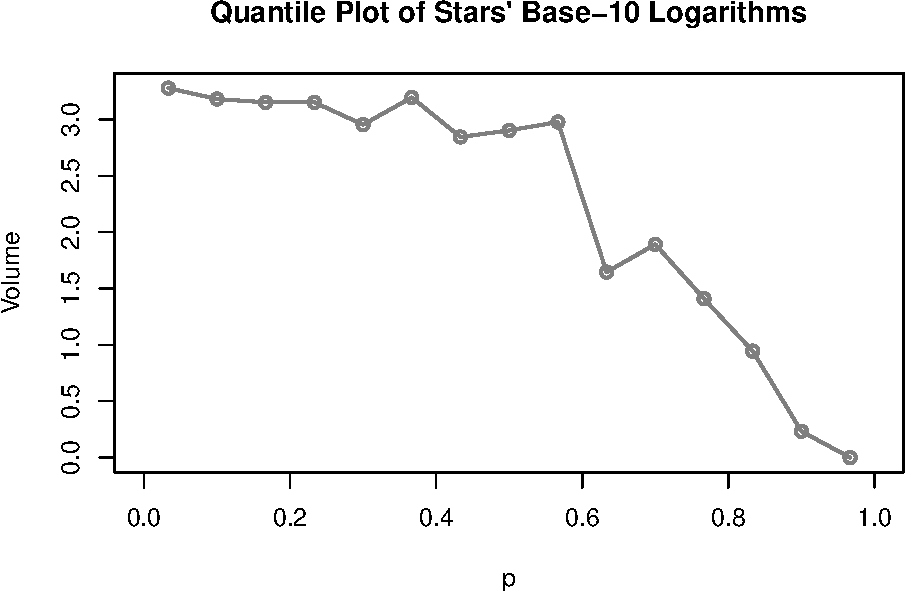
\includegraphics{a3_tests_files/figure-latex/unnamed-chunk-7-1.pdf}

\item 

\textbf{(4 marks)} Again construct a quantile plot of the logarithms of
the stellar radii \textbf{but} this time use base 2 logarithms. In the
same plot, overlay the quantiles for the base 10 logarithms. Explain how
and why the two sets of quantiles differ.

\begin{Shaded}
\begin{Highlighting}[]
\NormalTok{starLog2s =}\StringTok{ }\KeywordTok{log}\NormalTok{(starRadii[,], }\DataTypeTok{base=}\DecValTok{2}\NormalTok{)}
\NormalTok{ylims =}\StringTok{ }\KeywordTok{extendrange}\NormalTok{(}\KeywordTok{c}\NormalTok{(starLogs, starLog2s))}

\KeywordTok{plot}\NormalTok{(}\DataTypeTok{x =}\NormalTok{ p, }\DataTypeTok{y=}\NormalTok{starLogs, }
      \DataTypeTok{type=}\StringTok{"o"}\NormalTok{, }\DataTypeTok{lwd=}\DecValTok{2}\NormalTok{, }\DataTypeTok{col=}\StringTok{"red"}\NormalTok{,}
      \DataTypeTok{xlab=}\StringTok{"p"}\NormalTok{, }\DataTypeTok{ylab=}\StringTok{"Volume"}\NormalTok{,}
      \DataTypeTok{main=}\StringTok{"Quantile Plot of Stars' Logarithms"}\NormalTok{,}
      \DataTypeTok{xlim =}\KeywordTok{c}\NormalTok{(}\DecValTok{0}\NormalTok{,}\DecValTok{1}\NormalTok{), }\DataTypeTok{ylim=}\NormalTok{ylims)}

\KeywordTok{par}\NormalTok{(}\DataTypeTok{new =} \OtherTok{TRUE}\NormalTok{)}

\KeywordTok{plot}\NormalTok{(}\DataTypeTok{x =}\NormalTok{ p, }\DataTypeTok{y=}\NormalTok{starLog2s, }
      \DataTypeTok{type=}\StringTok{"o"}\NormalTok{, }\DataTypeTok{lwd=}\DecValTok{2}\NormalTok{, }\DataTypeTok{col=}\StringTok{"blue"}\NormalTok{,}
      \DataTypeTok{ylab=}\StringTok{"Volume"}\NormalTok{,}
      \DataTypeTok{xlim =}\KeywordTok{c}\NormalTok{(}\DecValTok{0}\NormalTok{,}\DecValTok{1}\NormalTok{), }\DataTypeTok{ylim=}\NormalTok{ylims)}
\end{Highlighting}
\end{Shaded}

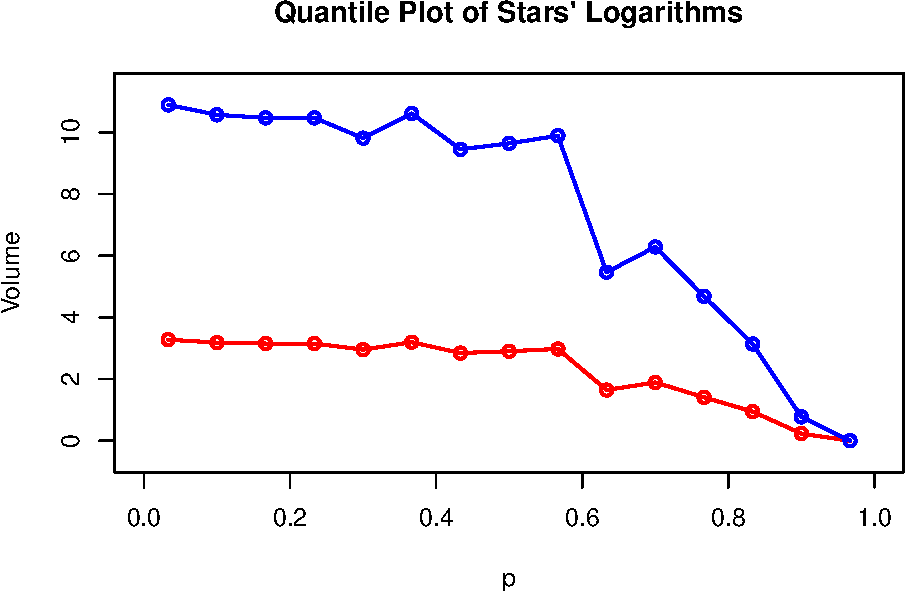
\includegraphics{a3_tests_files/figure-latex/unnamed-chunk-8-1.pdf}
\eenum
\eenum
\eenum


\end{document}
